\documentclass[12pt, a4paper]{report}
% for guidance, see phd_work/mnras_guide.pdf
%\setlength\parindent{0pt}

\usepackage[english]{babel}
\usepackage[utf8x]{inputenc}
\usepackage[T1]{fontenc}

%\documentclass[useAMS,usenatbib]{mn2e}
\newcommand{\aap}{A\&A}
\newcommand{\araa}{ARAA}
\newcommand{\mnras}{MNRAS}
\newcommand{\apjl}{ApJL}
\newcommand{\apjs}{ApJS}
\newcommand{\apj}{ApJ}
\newcommand{\aj}{ApJ}
\newcommand{\nat}{Nature}
\newcommand{\pasa}{PASA}
\newcommand{\pasj}{PASJ}
\newcommand{\pasp}{PASP}
\newcommand{\aapr}{A\&AR}
\newcommand{\procspie}{Proc. SPIE}
\newcommand{\apss}{Ap\&SS}
%\newcommand{\rsquo}{`}

\usepackage{graphicx}
%\usepackage{braket}
\usepackage[english]{babel}
\usepackage{upgreek}
\usepackage{graphicx}
\usepackage{float}
\usepackage{natbib}
\usepackage{amsmath}
\usepackage{amssymb}
\usepackage{tabularx,ragged2e,booktabs,caption}
\usepackage{graphicx} % for images
\usepackage[font=small]{caption}
\usepackage{setspace}
\usepackage{epstopdf}
\usepackage{subcaption}
\usepackage{url}

% ALW edit: FORMAT FOR INCLUDING PDF IMAGES!!!
% for guidance, see phd_work/grfguide.pdf
%\includegraphics[<options>]{filename.pdf}


%%%%%%%%%%%	Page layout settings that follow JMU regulations     %%%%%%%%%%

\setlength{\hoffset}{0mm}
\setlength{\oddsidemargin}{0mm}
\setlength{\evensidemargin}{0mm}

\setlength{\voffset}{-10mm}
\setlength{\topmargin}{0mm}
\setlength{\headheight}{10mm}
\setlength{\headsep}{10mm}

\setlength{\textheight}{220mm}
\setlength{\textwidth}{155mm}

\setlength{\columnsep}{10mm}
\setlength{\marginparsep}{0mm}
\setlength{\marginparwidth}{0mm}
\setlength{\footskip}{20mm}

\setlength{\parindent}{0.3in} % Size of indent at the start of a new paragraph - originally 0.0in
\setlength{\parskip}{0.0in} % Spacing between paragraphs - originally 0.1in

\usepackage[hang,splitrule]{footmisc}

\addtolength{\footskip}{0.5cm}
\setlength{\footnotemargin}{0.3cm}
\setlength{\footnotesep}{0.4cm}

\makeatletter
\let\splitfootnoterule=\pagefootnoterule
\makeatother

\begin{document}
\chapter{Theoretical background}
\section{Extinction definition} \label{extinc_desc}
Extinction is defined using the standard astronomical system of flux magnitudes. The difference between two generic flux measurements, $F_{1}$ and $F_{2}$, in magnitudes is expressed as:
\begin{equation}
\label{mags_def}
m_{1} - m_{2} = -2.5\log \left( \frac{F_{1}}{F_{2}} \right)
\end{equation}

where $m_{1}$ and $m_{2}$ are the measured flux magnitudes for $F_{1}$ and $F_{2}$, respectively. However, the flux of a source varies naturally with the distance to the observer (see Equation \ref{flux_def}). To account for this, the distances to the nearest stars were determined independently of their flux, by their parallax from Earth. The parallax $p$ of an object (measured in arcseconds in Equation \ref{parallax_eq}) is defined by the angular distance the object moves relative to the ``fixed'' background as the Earth moves a distance of 1AU (the average separation of the Sun and Earth during one complete orbit) perpendicular to the line-of-sight. This allows the distance, $d$, to be measured (in parsecs) using only the geometry of triangles, combined with the small-angle approximation, as:

\begin{equation}
d/\textnormal{pc} = \frac{1}{(p/\textnormal{arcsec})}
\label{parallax_eq}
\end{equation}

This gives each astronomical object two fundamental flux measurements. These are the apparent magnitude, $m$, and the absolute magnitude, $M$. The apparent magnitude is the flux magnitude of a source, as observed directly by the telescope. The absolute magnitude is the projected flux magnitude of the same source if it were to be placed at a distance of 10 parsecs (pc) from the telescope, thus accounting for the natural decrease in flux due to the distance between the source and the telescope. The relation between these quantities if there is zero extinction can be found by combining Equations \ref{flux_def} and \ref{mags_def}:
% In general, the extinction coefficient $A$ is defined relative to two ubiquitous astrophysical quantities.
\begin{equation}
\label{distance_modulus}
m - M = -2.5\log \left( \left(\frac{10\textnormal{pc}}{d}\right)^{2} \right) = 5\log\left(\frac{d}{\textnormal{pc}}\right) - 5
\end{equation}

The quantity ($m - M$) is known as the distance modulus, and, . It should be noted that the distance modulus in Equation \ref{distance_modulus} does not include extinction. To link the apparent magnitude to extinction, it is necessary to separate the distance modulus from the observed apparent magnitude, $m_{\textnormal{obs}}$. This can be done by defining the intrinsic apparent magnitude, $m_{0}$, such that:

\begin{equation}
\label{intrinsic_app_mag}
m_{0} - M = 5\log(d/\textnormal{pc}) - 5
\end{equation}

i.e., the distance modulus is solely dependent on the distance to the  sources. Therefore, the extinction $A$ can be defined as:

\begin{equation}
\label{bol_extinc}
A = m_{\textnormal{obs}} - m_{0}
\end{equation}

This fits with the definition of interstellar extinction given earlier, i.e. as the flux lost solely due to scattering and absorption in the interstellar medium.

However, as noted earlier, in astronomy it is infeasible to attempt observations by a single instrument at all wavelengths. Telescopes instead are generally purpose-built to study a single, relatively narrow wavelength range of the EM spectrum. Within this range, telescope observation ranges are further divided by filters or passbands, one of which is placed on their aperture at any given observation time. As shown in Figures \ref{ACS_response_funcs}-\ref{Gaia_response_funcs}, any single filter $X$ has a limited range of wavelengths for which it is able to detect flux. It can also be seen in these figures that the transmittance of the filter changes as a function of wavelength

\begin{equation}
f_{\lambda} = \frac{2hc}{\lambda^{5}\left(\exp\left({\frac{hc}{\lambda k_{B}T}}\right) - 1\right)}
\label{planck_bb}
\end{equation} 

****In this project, when comparing effects of different extinction treatments and, subsequently, when comparing observational datasets (with uncertainties in the values of their objects' stellar parameters and unknown extinction coefficients) to theoretical datasets via color-magnitude diagrams (CMDs), the most convenient format is to add the (theoretical) extinction coefficients to the theoretical dataset magnitudes (i.e., absolute magnitudes). As a result, the quantity from each dataset that is being compared in the CMDs is the absolute magnitude plus an extinction coefficient. If we label this quantity $M_{\textnormal{ext},X}$, we can define it bolometric as:

\begin{equation}
M_{\textnormal{ext},X} = M_{X} + A_{X}
\end{equation}

To measure a star's effective temperature, observers compare the star's observed flux in two filters at different wavelengths, typically in the UV-IR wavelength range. This is because a star with a higher effective temperature will be more luminous in every filter than a cooler star at the same position. This creates uncertainty if the distance measurement cannot be obtained independent of photometry. Therefore, observers utilise the colour index, which is defined as the difference between an object's magnitude in each of the two filters. ****If we compare the black body spectra in Figure****, it can be seen that the maximum monochromatic flux of the black body occurs at an increasingly shorter wavelength for increasingly hotter objects. This makes the object look bluer. The relationship between the wavelength at which the monochromatic flux is maximal and the black body temperature is quantified by Wien's displacement law.

The colour index is defined as the flux magnitude in the bluer (shorter-wavelength) filter minus that in the redder filter. For two filters $X$ and $Y$, with $X$ being bluer than $Y$, the colour index of observations made using them is:

\begin{align}
\begin{split}
(X-Y) &= m_{X} - m_{Y} \\
&= (m_{X,0} - m_{Y,0}) + (A_{X} - A_{Y}) \\
&= (X-Y)_{0} + E(X-Y)
\end{split}
\end{align}

where $(X-Y)_{0}$ is the intrinsic colour index of the object and $E(X-Y) = A_{X} - A_{Y}$ is known as the colour excess, but can also be denoted using ``reddening''. Due to the potential confusion of the term ``reddening'' between $A_{X}$ and $E(X-Y)$, the former will be referred to here as the ``extinction'' or ``extinction coefficient'' and the latter as the ``colour excess''. The colour excess represents the effect of extinction on the observed colour index. The colour excess is important because of the prominence of the intrinsic colour index in determining effective temperature. More negative values of $(X-Y)$ indicate bluer stars, with higher effective temperatures.

The most commonly-used colour index, employed as a reference for most optical observations, is the Johnson ($B-V$) index.

****Flambda is where t,g,z effects come into BC equations!!!

\section{Bolometric corrections} \label{BC_theory}
All the equations in Section ****, including those for extinction, are not useful when applied to telescopes, as any filter will only be able detect a small fraction of the stellar flux across all wavelengths (known as the bolometric stellar flux) that reaches the telescope, due to its response function. The missing information resulting from this observational constraint renders it difficult to determine the interstellar extinction. These constraints much be mitigated before an accurate value of the extinction coefficient can be determined. This mitigation is carried out by employing bolometric corrections.

The use of bolometric corrections requires the detailed knowledge of stellar spectra least susceptible to significant extinction, i.e., nearby stars with high apparent fluxes. Only with complete knowledge of the spectrum from a reference star can the true spectrum of a distant star with unknown extinction be calculated. The spectra of these stars can be computed by using a grid of predicted fluxes from a stellar atmosphere model, the grid being composed of the stellar parameters known to change emission in stellar atmospheres. These are effective temperature, surface gravity and metallicity. For all filter systems studied in this project, the nearby star Vega ($\alpha$ Lyr) was used as the reference object. Using Vega as the reference star is the most well-known approach to calibration \citep{2014MNRAS.444..392C}.

The effective temperature ($T_{\textnormal{eff}}$) of a star is defined as the temperature of a black body which produces the same bolometric flux as that produced by the star. This approximation is valid because all stars have been observed to have spectra that closely resemble those of black bodies, with the notable exception of atmospheric absorption lines.

\begin{equation}
L = 4 \pi R^{2} \sigma_{SB} T_{\textnormal{eff}}^{4}
\label{Teff_def}
\end{equation}

\begin{figure}[h]
\begin{center}
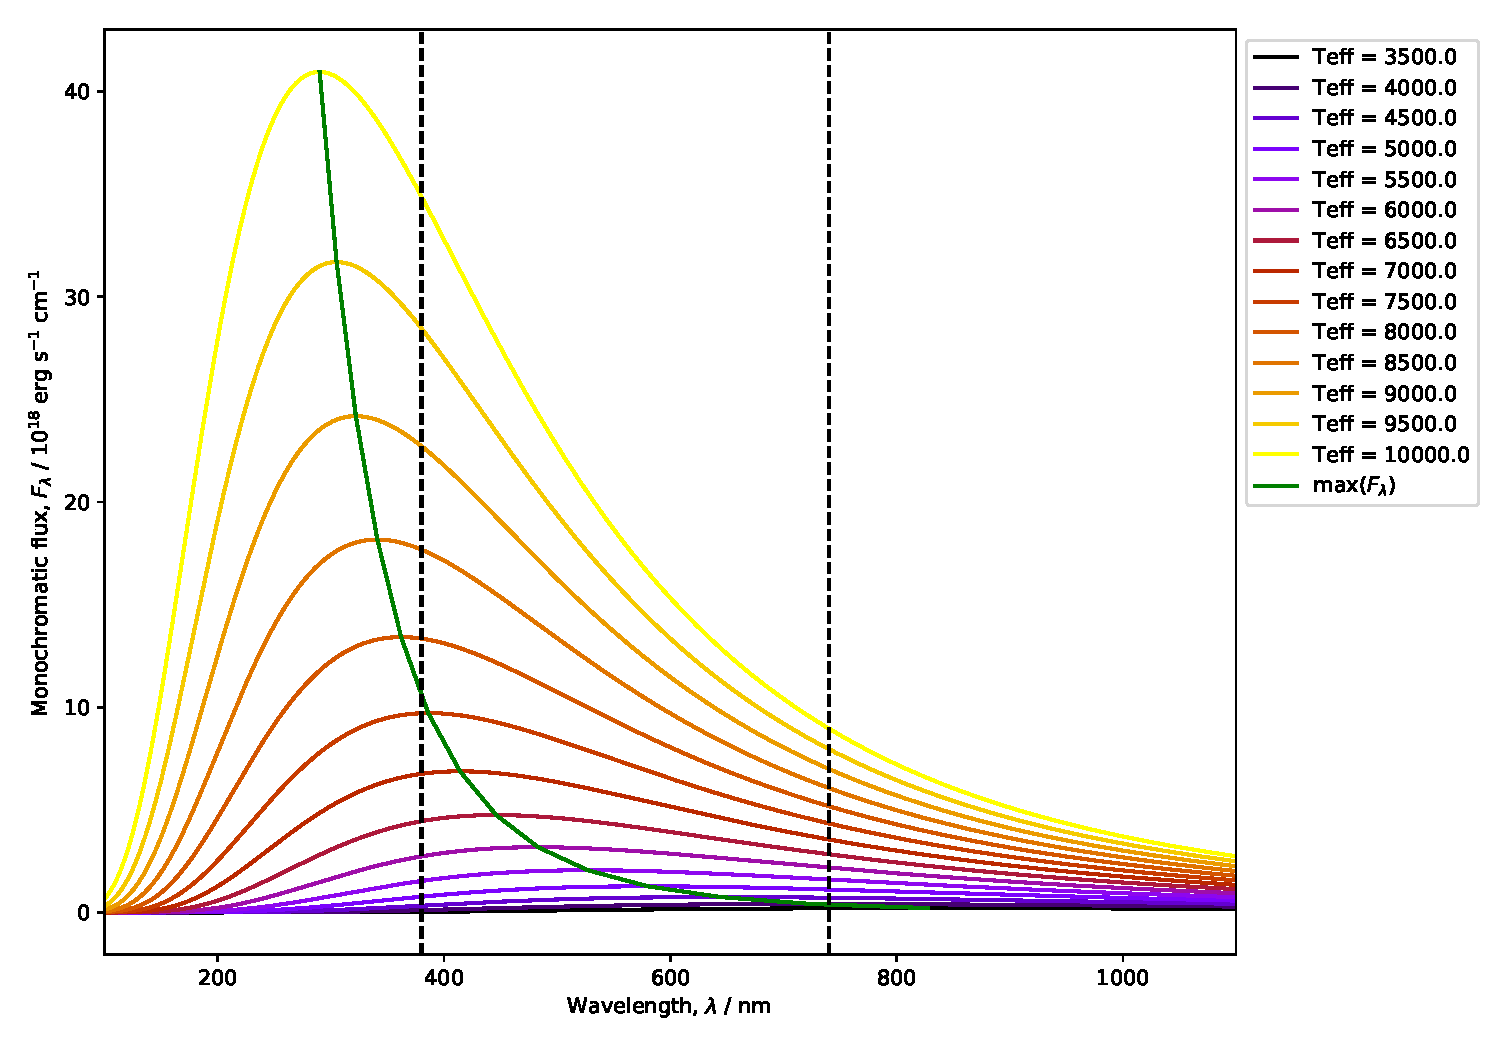
\includegraphics[scale=0.5]{blackbody_teff_illustration.pdf}
\caption{****Monochromatic flux of a black body for different stellar effective temperatures. The black dashed lines mark the approximate limits of the visible part of the EM spectrum. The green curve represents the distributed of the maxima for the other curves.}
\label{planck_curve}

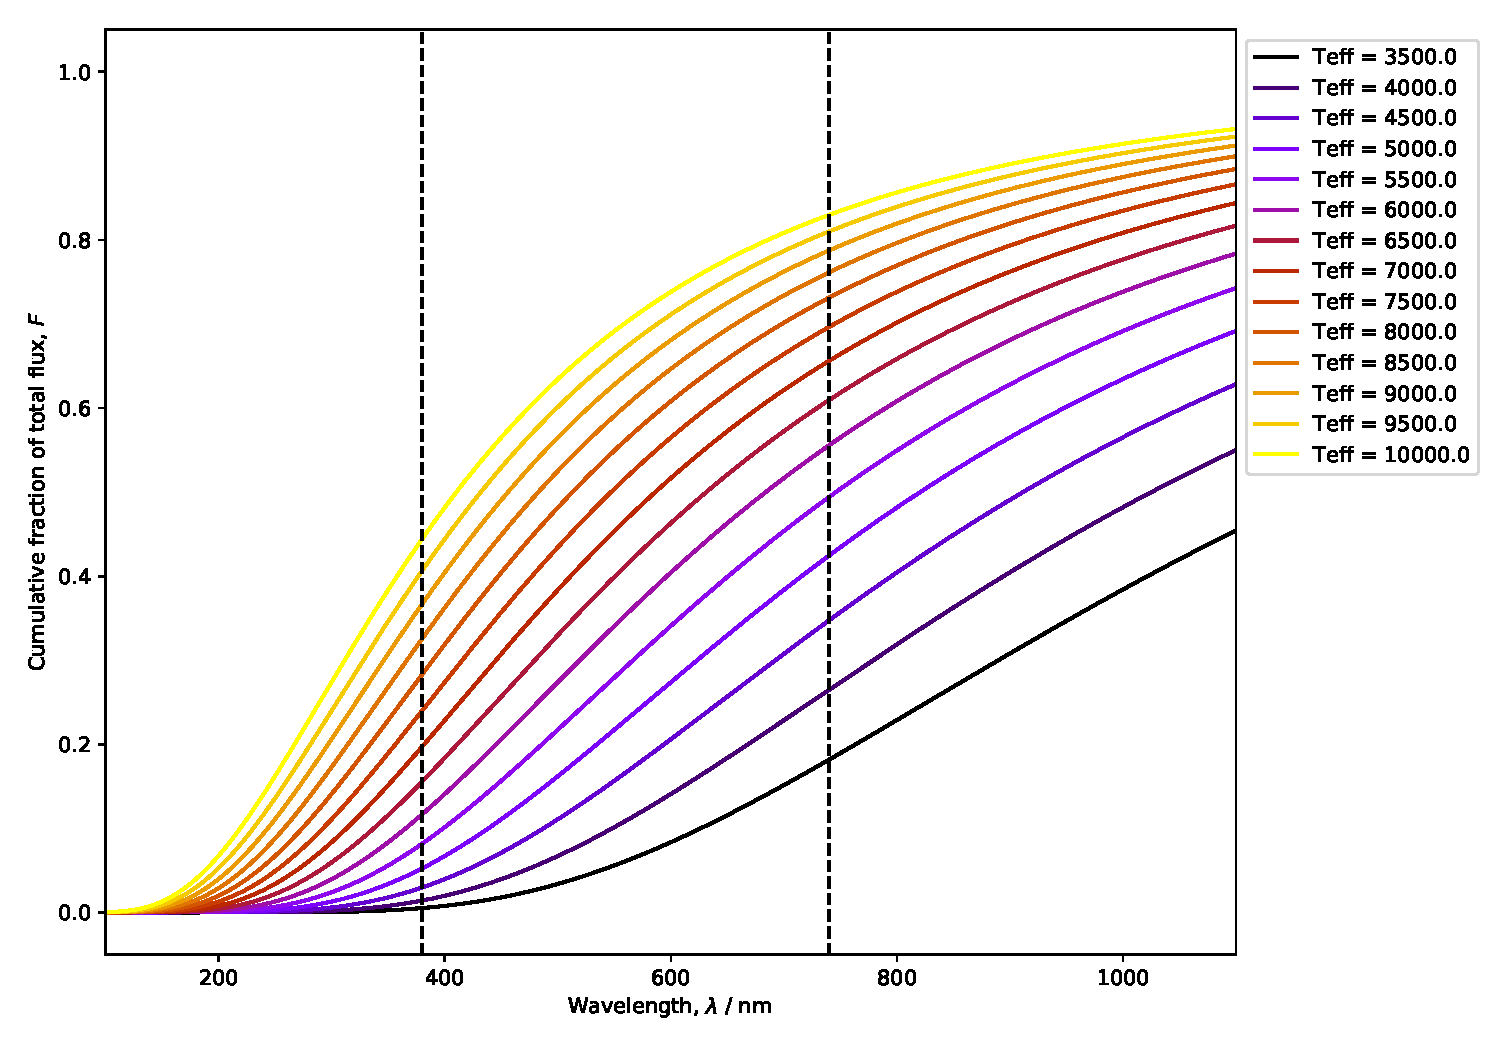
\includegraphics[scale=0.5]{cumulative_blackbody_teff_illustration.pdf}
\caption{Cumulative fraction of the total flux of a black body for different stellar effective temperatures. The black dashed lines mark the approximate limits of the visible part of the EM spectrum.}
\label{cumulative_planck_curve}
\end{center}
\end{figure}

Effective temperature has an effect on interstellar extinction due to its strong effect on the stellar luminosity and, hence, the flux. For a higher flux, more photons are likely to interact with the ISM, hence a higher extinction coefficient.

The metallicity of a star is defined as the fractional abundance of heavy elements, often approximated by iron alone, relative to the star's hydrogen abundance, compared to that of the Sun. The abundances are determined by the strength of the elements' characteristic atomic absorption lines in the stellar spectra.

\begin{equation}
\textnormal{[Fe/H]} = \log(N_{\textnormal{Fe}}/N_{\textnormal{H}}) - \log(N_{\textnormal{Fe},\odot}/N_{\textnormal{H},\odot})
\label{FeH_def}
\end{equation}

Since the output is logarithmic, a value of [Fe/H] = 0 indicates solar metallicity. An increase in metallicity would cause the corresponding absorption lines to be stronger, thus reducing the observable flux. An increased metallicity also implies an increase in abundance of sub-ferrous metals. The presence of more nuclear species, each with unique absorption line configurations, inevitably creates more observable lines, further increasing the apparent extinction in the spectral flux.

The definition of the stellar surface gravity $g$ is simply the value of the standard Newtonian gravitational acceleration, applied to the stellar surface (the mass is the total stellar mass, $M_{*}$, and the distance is the stellar radius, $R_{*}$):

\begin{equation}
g = \frac{GM_{*}}{R_{*}^{2}}
\label{gravity_def}
\end{equation}

A higher surface gravity represents a surface with a higher atomic number density. This environment produces a shorter mean free path for photons overall, meaning a smaller collision timescale. If the timescale is sufficiently small, the limit provided by Heisenberg's Uncertainty Principle causes an increase in the uncertainty of the energy absorbed by the atomic electron during the interaction with the photon:

\begin{equation}
\Delta E \Delta t \geq \hbar/2
\label{heisenberg}
\end{equation}

This effect, known as ``pressure broadening'', causes a symmetrical distribution of absorption energies (and wavelengths) about the normal emission energy for that particular atomic state. This means fewer photons pass through the surface, thereby reducing the surface flux.

After accounting for a general extinction effect on an object's emission, its apparent magnitude in a given filter $X$ (i.e. wavelength range, which we define as increasing from $\lambda _{1}$ to $\lambda _{2}$) is given by:

\begin{equation}
m_{X} = -2.5 \log_{10} \left(\frac{ \int_{\lambda_{1}}^{\lambda_{2}} f_{\lambda} \left( 10^{-0.4 A_{X,\lambda}} \right) S_{\lambda} d\lambda }{ \int_{\lambda_{1}}^{\lambda_{2}} f_{\lambda}^{0} S_{\lambda} d\lambda }\right) + m_{X}^{0}
\label{app_mag_def}
\end{equation}

where $f_{\lambda}$ represents the monochromatic flux at a given wavelength $\lambda$ at the observer distance, $A_{X,\lambda}$ is the extinction value as a function of wavelength, $S_{\lambda}$ represents the filter response function and $f_{\lambda}^{0}$ and $m_{X}^{0}$ represent the monochromatic flux and apparent magnitude, respectively, of a known reference object in $X$.

%Since our goal, ultimately, is to document potential effects of fundamental stellar properties upon observables, we need to connect the observational and idealised scenarios, for which we use bolometric corrections.

To derive the equation linking a bolometric correction with the extinction parameter, we start with the definition of a bolometric correction in a filter $X$, which is denoted by $BC_{X}$:

\begin{equation}
BC_{X} \equiv M_{\textnormal{bol}} - M_{X}
\label{BC_def}
\end{equation}

where $M_{X}$ is the absolute magnitude of the object in $X$ and $M_{\textnormal{bol}}$ is its (predicted) absolute bolometric magnitude, defined relative to the Sun using:

\begin{equation}
M_{\textnormal{bol}} = M_{\textnormal{bol},\odot} - 2.5 \log_{10} \left( \frac{4\pi R^{2}F_{\textnormal{bol}}}{L_{\odot}} \right)
\label{mbol_sun}
\end{equation}

where  $F_{\textnormal{bol}}$ is the bolometric stellar flux at its surface, $R$ is the stellar radius, $M_{\textnormal{bol},\odot}$ is the solar absolute bolometric magnitude, which is assumed in this work to have a value of 4.75 and $L_{\odot}$ is the solar luminosity, for which a value of $3.844 \times 10^{33}$ erg s$^{-1}$ is used. Bolometric corrections can be expressed as a function of extinction using the universal definition of $M_{X}$ in terms of $m_{X}$ and the distance $d$ to the source:

\begin{equation}
M_{X} = m_{X} - 2.5 \log_{10}\left( \left( \frac{d}{10 \textnormal{pc}} \right)^{2} \right),
\label{abs_mag_def}
\end{equation}

together with the equation $f_{\lambda}d^{2}=F_{\lambda}R^{2}$, where $F_{\lambda}$ is the monochromatic flux at $\lambda$ at the stellar surface. This gives the final function for a bolometric correction for filter $X$:

\begin{align}
\begin{split}
BC_{X} &= M_{\textnormal{bol},\odot} - m_{X}^{0} - 2.5 \log_{10} \left( \frac{4\pi R^{2}F_{\textnormal{bol}}}{L_{\odot}} \right) \\
&+ 2.5 \log_{10} \left( \frac{\int_{\lambda_{1}}^{\lambda_{2}} F_{\lambda} \left( 10^{-0.4 A_{X,\lambda}} \right) S_{\lambda} d\lambda}{\int_{\lambda_{1}}^{\lambda_{2}} f_{\lambda}^{0} S_{\lambda} d\lambda} \right)
\label{BC_extinc}
\end{split}
\end{align}

For a filter $X$, the extinction parameter $A_{X} = A_{X,\lambda}$ must be calibrated relative to a known value. In this work we will input a value of the extinction in the well-studied Johnson-$V$ filter, $A_{V}$. To extract $A_{X}$, we use the simple relation:

\begin{equation}
A_{X} = \left( \frac{A_{X}}{A_{V}} \right) A_{V}
\label{ratio_eq}
\end{equation}

together with the chosen value of $A_{V}$ (for this project the values were $A_{V} =$ 0, 1 - note that $BC_{X}(A_{V}=0)$ effectively assumes no extinction in any filter, via Equation ), before taking the difference between the two $BC_{X}(A_{V})$, giving the following equation:

\begin{align}
\begin{split}
BC_{X}(0) - BC_{X}(A_{V}) &= 2.5 \log_{10} \left( \frac{\int_{\lambda_{1}}^{\lambda_{2}} F_{\lambda}  S_{\lambda} d\lambda}{\int_{\lambda_{1}}^{\lambda_{2}} F_{\lambda}\left( 10^{-0.4 \left(A_{X,\lambda}/A_{V}\right)A_{V}} \right) S_{\lambda} d\lambda} \right)
\label{BCs_diff}
\end{split}
\end{align}
%\\ &\approx \left(A_{X}/A_{V}\right)A_{V}

****average over the wavelength interval $[\lambda_{1},\lambda_{2}]$ which is a valid assumption \citep{2014MNRAS.444..392C}, as the CCM relations, which were derived using data from stars observed in the Johnson broad-band filters, themselves were. Due to the nature of the filters' bandpasses, the CCM relations overestimate the extinction in the near-IR and blue-visible Johnson filters
%\citep{1999fitzpatrick.

\bibliographystyle{mnras} % unsrtnat
\bibliography{mphil_thesis}

\end{document}